\section{Fluxo de avaliação de vida à fadiga sem a ferramenta}\label{sec:workflow}
% TODO: Sugestão: isso poderia aparecer no cap1, seção problemática.
% TODO: Seria importante apresentar este fluxo de uma forma mais conceitual, sem ser específico no uso do ABAQUS ou FatFree. Quando for necessário comentar sobre essas ferramentas, poderia fazer isto citando-as como exemplos do fluxo conceitual.


Baseado nos estudos e oficinas realizados para o desenvolvimento deste trabalho, pôde-se estabelecer que a análise de vida à fadiga em dutos em vão-livre compreende o fluxograma apresentado na \autoref{fig:fluxograma}. % chktex 19

\begin{figure}[!ht]
    \centering
    \caption{Fluxo de avaliação de vida à fadiga em dutos em vão-livre.}\label{fig:fluxograma}
    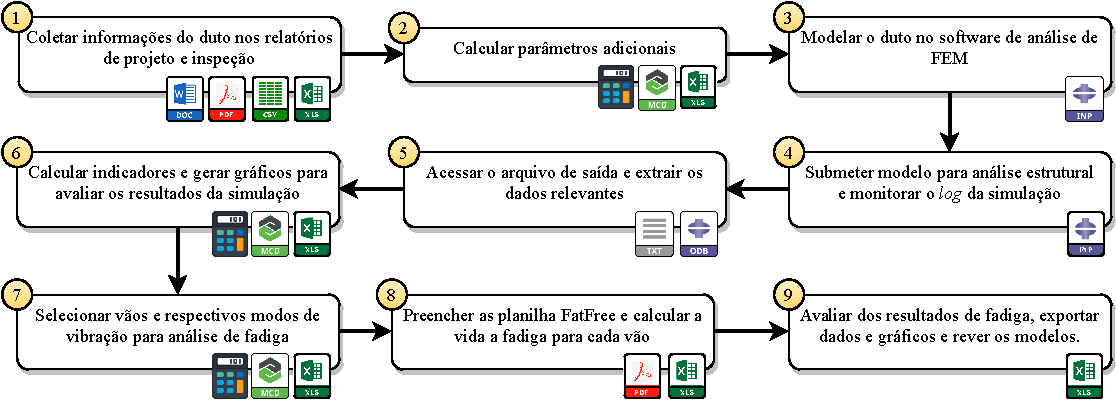
\includegraphics[width=\textwidth]{imagens/fluxograma.pdf}
    \fonte{Autor (2020)}
\end{figure}

A seguir, uma breve descrição de cada item:

% TODO Essas suas afirmações não estão claras para mim. Seria importante explicar de uma forma mais organizada no texto o que você está chamando de pós-processamento. Essas últimas frases estão bem ruins. Melhor fazer um outro fluxograma posteriormente indicando quais são as etapas envolvidas em cada uma das fases de pré, análise e pós-processamento. Acho que fica melhor.

\begin{enumerate}[label= (\arabic*)]
    \item Nesta etapa, o profissional reúne as informações básicas para construção dos modelos e outros dados usados em cálculos posteriores, por exemplo: as cotas do perfil do duto e batimetria obtidas na inspeção, geometria e propriedades dos materiais das camadas que compõem seção do duto, os parâmetros do solo, dados metaoceanográficos, os coeficientes de segurança e outras constantes físicas, posição e tipos de suportes\footnote{restrições nodais ou apoios} ao longo do duto;
    Essa tarefa envolve analisar uma série de documentos (\texttt{.doc}, \texttt{.pdf}, etc) em busca desses valores, dispostos de forma não estruturada. Quando estruturados, em forma de arquivos CSV ou planilhas, por exemplo, é necessário ainda manipular esses dados de modo a extrair somente a informação necessária e/ou convertê-las no formato apropriado. Um exemplo disso são os dados de batimetria, que precisam ser convertidos nas coordenadas dos nós de uma malha de elementos finitos no formato de um arquivo \texttt{.inp} --- no caso do ABAQUS. De posse desses dados, pode-se iniciar a fase de pré-processamento.
    \item Uma vez que nem todos os dados a serem utilizados estão de acordo com as especificações dos softwares a serem empregadas nas análises numéricas, ainda é necessários manipular alguns desses valores, seja calculando constantes ou convertendo unidades. Para isso, geralmente utiliza-se softwares de planilhas e/ou folhas de cálculos (Microsoft Excel, MathCad, Maple, etc.). Esta etapa corresponde ao início da primeira fase de pré-processamento de dados;
    \item Com todos os dados em mãos, é necessário transformá-los em um modelo numérico no software de elementos finitos, via interação com mouse e teclado (GUI), ou criando arquivos de entrada. Embora a reutilização de arquivos de entrada previamente criados facilite essa tarefa, nem todos os trechos desses arquivos são suficientes ou podem ser reaproveitados. Essas limitações são frequentes em trechos do arquivo que precisam ser repetidos a depender da quantidade de certas entidades no modelo (suportes, por exemplo). Ao fim desta etapa, encerra-se o pré-processamento dos dados;
    \item Por mais simples que seja submeter o modelo para análise na maioria dos softwares de simulação numérica por elementos finitos (alguns cliques via GUI ou um comando via CLI\footnote{\textit{Command Line Interface}: interface de linha de comando}), as análises costumam levar horas e envolver execuções sucessivas a fim de realizar intervenções no modelo que não podem ser modeladas previamente. Dessa forma, torna-se necessário o monitoramento do progresso da simulação. Esta etapa compreende a primeira parte do processamento propriamente dito;
    \item Uma vez concluída a simulação via Elementos Finitos, é necessário analisar os resultados antes do pós-processamento. Por vezes, é preciso extrair as informações que estão armazenadas em arquivos proprietários (como \texttt{.odb}, no caso do ABAQUS), utilizando, para isto, as funcionalidades das ferramentas dos próprios pacotes de software de elementos finitos. Esta tarefa, geralmente feita via GUI, costuma ser repetitiva e pode levar de alguns minutos ou horas. Esta etapa inicia parte do pós-processamento da análise de elementos finitos;
    \item De posse dos resultados, é necessário calcular (e muitas vezes visualizar em gráficos) alguns indicadores a fim de avaliar a qualidade dos resultados. Embora poderosos, estes softwares ainda carecem de gráficos mais interativos, como possibilidades de manipulações diretas importantes, tais como ampliação e translação dos mesmos através do uso do mouse. Esta etapa encerra o pós-processamento da análise de elementos finitos;
    \item Na metodologia presente na \dnvf105 --- abordada na \autoref{sec:multimode} --- o cálculo de fadiga é baseada em modelos de resposta, portanto, é necessário calcular a resposta de cada modo para as várias condições de carregamento ambiental, o que a torna impraticável sem automação. Embora a  \fatfree realize estas operações, dentre as dezenas de modos obtidos por solução modal na análise de elementos finitos costumam aparecer modos espúrios. Dessa forma, antes de realizar a análise na \fatfree, é necessário escolher dentre os modos de vibração obtidos na simulação numérica aqueles que mais contribuem para fadiga. Esta tarefa costuma ser feita via inspeção visual, observando a forma dos modos, mas é uma prática pouco precisa e subjetiva;
    \item Uma vez selecionados os modos a serem usados para cálculo de fadiga, é necessário o preenchimento da planilha com os dados de deslocamentos ou tensão adimensionalidos pelo diâmetro de cada modo, o que consiste em algumas centenas de valores. Além disso, é necessário preencher muitas outras informações referentes a geometria e propriedades dos materiais da seção do duto, parâmetros do solo, coeficientes de segurança e condições de carregamento em várias páginas diferentes. Com todos os dados preenchidos e opções selecionadas nos controles da planilha, pode-se a chamar a rotina que calcula os resultados de fadiga;
    \item Finalmente, os dados de fadiga pode ser analisados e exportados para outras ferramentas a fim de gerar gráficos e relatórios.
\end{enumerate}
